\section{Результаты и обсуждение}

Ранее было показано~\cite{2019, Shelkovnikov2019}, что формильные производные триарилпиразолинов, содержащих полифторфенильные остатки в положениях 5 или 3 пиразолинового цикла, могут служить эффективными донорами в синтезе сопряженных донорно-акцепторных хромофоров с поглощением при 720--760~нм.
В развитие этой тематики была поставлена задача синтеза Д-А хромофоров c использованием декафторзамещенных производных триарилпиразолина. Наличие двух пентафторфенильных групп дает дополнительные возможности для модификации донорного фрагмента.

Альдегид~\cmpd{decafluoropyrazoline_CHO} был наработан по литературной методике~\cite{2016a,2010}.
Его получение представляет собой многостадийный процесс~(\ref{sch:decafluoropyrazoline_synthesis}).
Альдольно-кротоновой конденсацией пентафторацетофенона~\cmpd{perfluorobenzacetophenone} с пентафторбензальдегидом~\cmpd{perfluorobenzaldehyde} получали декафторхалкон~\cmpd{decafluorochalcone}, который переводили в пиразолин~\cmpd{decafluoropyrazoline} конденсацией с фенилгидразином.
Далее кольцо в положении 1 пиразолина~\cmpd{decafluoropyrazoline} формилировали реакцией Вильсмайера, получая альдегид~\cmpd{decafluoropyrazoline_CHO}.
\begin{scheme}[h!]
    \centering
    \begin{overpic}{sections/results/img/decafluoropyrazoline_synthesis.eps}
        \put(7, 40){\cmpd{perfluorobenzacetophenone}}
        \put(30, 40){\cmpd{perfluorobenzaldehyde}}
        \put(71, 40){\cmpd{decafluorochalcone}}
        \put(82, 7){\cmpd{decafluoropyrazoline}}
        \put(22, 8){\cmpd{decafluoropyrazoline_CHO}}
    \end{overpic}
    % \caption{Синтез декафторпиразолина}
    \caption{}
    \label{sch:decafluoropyrazoline_synthesis}
\end{scheme}

% \subsection{Красители с остатком 4-гидроксипиперидина}

\subsection{\nohyphens{Взаимодействие формилированного декафтортриарилпиразолина с бинуклеофилами}}

Далее атом фтора в \emph{пара}-положении обоих колец замещали на бифункциональный нуклеофил: 4-гидроксипиперидин или пиперазин~(\ref{sch:decafluoropyrazoline_substitution}).
При~\SI{60}{\celsius} реакция замещения фтора в обеих пентафторфенильных группах на остатки 4-гидроксипиперидина не идет до конца, в смеси присутствует примесь исходного соединения. Поэтому реакционную смесь выдерживали при~\SI{100}{\celsius}. Из реакционной смеси были выделены два соединения~--- целевой альдегид с двумя гидроксипиперидиновыми остатками и альдегид, содержащий в одном из колец диметиламиногруппу. Положение диметиламиногруппы было установлено реакцией альдегида~\cmpd{decafluoropyrazoline_CHO} с недостатком 4-гидроксипиперидина, при которой незамещенным и, следовательно, менее реакционноспособным оказалось перфторфенильное кольцо в положении 5. \todo{РСА}

\begin{scheme}[h!]
    \centering
    \begin{overpic}{sections/results/img/fluorine_substitution.eps}
        \put(7, 26.5){\cmpd{decafluoropyrazoline_CHO}}
        \put(47, 5){\cmpd{decafluoropyrazoline_substituted.piperidine}}
        \put(85, 5){\cmpd{decafluoropyrazoline_substituted.Me2N}}
    \end{overpic}
    \caption{}
    \label{sch:decafluoropyrazoline_substitution}
\end{scheme}

Спектры ЯМР продукта~\cmpd{decafluoropyrazoline_substituted.piperidine} явно отражают его структуру.
В спектре ЯМР~\ce{^1H} наблюдаются сигнал альдегидного протона; сигналы системы~\emph{A{A\chemprime}BB\chemprime} \emph{пара}-фениленового кольца; три дублета дублетов, соответствующие системе~\emph{ABX} пиразолинового кольца; в сильном поле~---мультиплеты, соответствующие протонам пиперидиногруппы, в том числе сложный мультиплет, принадлежащий протону \ce{CH-OH}.
Спектр~\ce{^19F} также имеет характерный вид и содержит уширенный синглет, который соответствует атомам фтора в \emph{орто}-положении кольца в 5 положении пиразолина.
Считается, что это уширение связано с взаимодействием этих атомов фтора с ароматическим кольцом в 1 положении пиразолина.



Первоначально пиперазин вводили в тех же условиях, что и 4-гидроксипиперидин при этом из реакционной смеси был выделен только продукт олигомеризации (сшивки) по пиперазиновым группам. При проведении реакции при температуре \SI{80}{\celsius} и десятикратном избытке пиперазина в реакционной смеси удается выделить продукт замещения обоих атомов фтора на остатки пиперазина в смеси с, предположительно, продуктом замещения одного из атомов фтора на диметиламиногруппу, аналогично реакции с 4-гидроксипиперидином. \todo{уточнить}

\begin{scheme}
    \begin{overpic}{sections/results/img/oligo.eps}
        \put(7, 15){\cmpd{decafluoropyrazoline_CHO}}
    \end{overpic}
    \caption{}
    \label{sch:oligo}
\end{scheme}


\subsection{Методика введения разделительного блока}
После этого гидроксигруппу альдегида~\cmpd{decafluoropyrazoline_substituted.piperidine} ацилировали хлористым бензоилом~(\ref{sch:ac_cond}).
Были испытаны два подхода: бензоилирование большим избытком хлористого бензоила  и бензоилирование с катализом~\ac{dmap} и стехиометрическим количеством  хлористого бензоила.
В результате было обнаружено, что использование~\ac{dmap} позволяет сократить время реакции с 6--8 часов до 2 в случае хлористого бензоила и требует гораздо меньшего избытка хлорангидрида~(1.25~экв. против 3~экв. при проведении реакции без катализатора).

О полном ацилировании \ce{OH}-групп можно судить по смещению сигнала протонов \ce{CH-OH} в слабое поле.

\begin{scheme}[ht]
    \centering
    \begin{overpic}{sections/results/img/ac_cond.eps}
        \put(8.5, 50){\cmpd{decafluoropyrazoline_substituted.piperidine}}
        \put(70, 37){\cmpd{decafluoropyrazoline_piperidine_benzoyl}}
        \put(27, 17){\cmpd{decafluoropyrazoline_piperidine_DCIF.benzoyl}}
    \end{overpic}
    \caption{}
    \label{sch:ac_cond}
\end{scheme}

Также мы исследовали альтернативную последовательность реакций: конденсацию альдегида~\cmpd{decafluoropyrazoline_substituted.piperidine} с дицианоизофороном и последующее ацилирование полученного \mbox{\ce{OH}-красителя}~\cmpd{decafluoropyrazoline_DCIF.piperidine}~(\ref{sch:cond_ac}).


\begin{scheme}[ht]
    \centering
    \begin{overpic}{sections/results/img/cond_ac.eps}
        \put(3, 74){\cmpd{decafluoropyrazoline_substituted.piperidine}}
        \put(40, 55){\cmpd{decafluoropyrazoline_DCIF.piperidine}}
        \put(83, 74){\cmpd{decafluoropyrazoline_piperidine_DCIF.{benzoyl, TAFS, TATBS}}}
        \put(23, 8){\cmpd{pentafluoropyrazoline_DCIF.piperidine}}
        \put(76, 6){\cmpd{pentafluoropyrazoline_piperidine_DCIF.{benzoyl, TAFS, TATBS, MATBS}}}
    \end{overpic}
    \caption{}
    \label{sch:cond_ac}
\end{scheme}

При сопоставимых выходах на стадии ацилирования более выгодным является подход с конденсацией и последующим ацилированием, поскольку он позволяет использовать меньшее количество хлорангидрида, получение которого представляется собой значительную сложность. В итоге оптимизированная последовательность реакций и методика ацилирования позволила снизить требуемое количество ацилирующего реагента и повысить выход~(для соединения~\cmpd{pentafluoropyrazoline_piperidine_DCIF.benzoyl} без катализатора выход составляет 6--\SI{15}{\percent}~\cite{2019}).

\begin{table}[]
    \centering
    \caption{}
    \label{tab:acylation_bis}
    \begin{small}
        \begin{threeparttable}
            \begin{tabular}{cccccccc}
                \toprule{}
                \textbf{№} & \textbf{Субстрат}                                  & \textbf{\thead{Экв.                                                                                                       \\реагента}} & \textbf{Продукт}                                     & \textbf{Условия}                    & \textbf{\makecell{Время\\реакции,~ч}} & \textbf{Выход, \%} \\
                \midrule
                1          & \cmpd{decafluoropyrazoline_substituted.piperidine} & 6                   & \cmpd{decafluoropyrazoline_piperidine_benzoyl}      & \ce{PhH}, \ce{NEt3}                 & 24 & 74 \\
                2          & \cmpd{decafluoropyrazoline_substituted.piperidine} & 2.5                 & \cmpd{decafluoropyrazoline_piperidine_benzoyl}      & \ce{PhH}, \ce{NEt3}, \ac{dmap}      & 6  & 74 \\
                3          & \cmpd{decafluoropyrazoline_DCIF.piperidine}        & 3                   & \cmpd{decafluoropyrazoline_piperidine_DCIF.benzoyl} & \ce{PhH}, \ce{NEt3},      \ac{dmap} & 2  & 25 \\
                4          & \cmpd{decafluoropyrazoline_DCIF.piperidine}        & 3                   & \cmpd{decafluoropyrazoline_piperidine_DCIF.TAFS}    & \ce{PhH}, \ce{NEt3},      \ac{dmap} & 2  & 30 \\
                5          & \cmpd{decafluoropyrazoline_DCIF.piperidine}        & 3                   & \cmpd{decafluoropyrazoline_piperidine_DCIF.TATBS}   & \ce{PhH}, \ce{NEt3},      \ac{dmap} & 6  & 55 \\
                \bottomrule
            \end{tabular}
        \end{threeparttable}
    \end{small}
\end{table}

В спектре ЯМР \ce{^1H} соединения \cmpd{{decafluoropyrazoline_DCIF.piperidine}} характеристическими являются сигналы \emph{AB}-системы двойной связи с \ac{J} около \SI{15}{\hertz}, что указывает на \emph{E}-конфигурацию двойной связи, синглет при \SI{6.72}{\ppm}, соответствующий протону при двойной связи дицианоизофорона, два синглета при 2.61 и \SI{2.55}{\ppm}, принадлежащих \ce{CH2} группам дицианоизофорона и синглет при \SI{1.04}{\ppm}, принадлежащий двум метильными группам дицианоизофорона.

Мы обнаружили, что в реакции бензоилирования~\cmpd{decafluoropyrazoline_DCIF.piperidine} при длительной выдержке реакционной смеси вместо пиразолина~\cmpd{decafluoropyrazoline_piperidine_DCIF.benzoyl} образуется соответствующий пиразол.
На образование пиразола указывает отсутствие в \ce{^1H} ЯМР спектре сигналов \emph{ABX}-системы пиразолина и отсутствие в спектре \ce{^19F} уширенного синглета.

Также мы наблюдали окисление пиразолина~\cmpd{decafluoropyrazoline_piperidine_DCIF.benzoyl} в пиразол даже при кратковременной выдержке в темноте в хлорированных растворителях~(\ce{CH2Cl2} и \ce{CDCl3}).
При этом для предшественника соединения~\cmpd{decafluoropyrazoline_piperidine_DCIF.benzoyl}~--- альдегида~\cmpd{decafluoropyrazoline_substituted.piperidine} окисления не наблюдалось даже при длительной выдержке в хлороформе на свету.
Это может быть связано с предполагаемым механизмом окисления~(\ref{sch:light_oxidation} на стр.\,\pageref{sch:light_oxidation}); введение в молекулу акцептора упрощает образование цвиттерионной структуры, играющей ключевую роль в процессе окисления.
Таким образом, наилучшая стратегия при синтезе и очистке производных альдегида~\cmpd{decafluoropyrazoline_substituted.piperidine}~--- избегать хлорсодержащих растворителей.\todo{как-то криво}

\subsection{Синтез красителей}

По оптимизированной методике~(\ref{sch:cond_ac}) мы синтезировали производные соединений~\cmpd{decafluoropyrazoline_DCIF.piperidine} и~\cmpd{pentafluoropyrazoline_DCIF.piperidine}\todo{Написать?} с разделительными блоками~(\ref{fig:dendroids})~--- эфиры~\cmpd{decafluoropyrazoline_piperidine_DCIF.{benzoyl, TAFS, TATBS}} и~\cmpd{pentafluoropyrazoline_piperidine_DCIF.{benzoyl, TAFS, TATBS, MATBS}}.
В целом, реакция ацилирования идет достаточно быстро и с хорошим выходом~(\ref{tab:acylation_bis}, \ref{tab:acylation_mono}), однако в случае соединения~\cmpd{pentafluoropyrazoline_piperidine_DCIF.MATBS} выход продукта составляет всего \SI{7.5}{\percent}.

\begin{figure}[h!]
    \centering
    \begin{overpic}{sections/results/img/dendroids.eps}
    \end{overpic}
    \caption{Структуры использованных разделительных блоков}
    \label{fig:dendroids}
\end{figure}

Это может быть связано с тем, что хлорангидрид является стерически затрудненным, а следовательно, затруднен подход OH-группы к карбонильной группе.
Для получения соединения~\cmpd{pentafluoropyrazoline_piperidine_DCIF.MATBS} мы использовали несколько вариаций общей методики: увеличение времени реакции, замена растворителя с бензола на ацетонитрил, проведение реакции при повышенной температуре с нагревом микроволновым излучением, однако это не привело к повышению выхода.

\begin{table}[h!]
    \centering
    \caption{Результаты ацилирования соединения~\cmpd{pentafluoropyrazoline_DCIF.piperidine}}
    \label{tab:acylation_mono}
    \begin{small}
        \begin{threeparttable}
            \begin{tabular}{ccccccc}
                \toprule{}
                \textbf{№} & \textbf{Реагент} & \textbf{\thead{Экв.                                                                                                            \\реагента}} & \textbf{Продукт} & \textbf{Условия}          & \textbf{\makecell{Время\\реакции,~ч}} & \textbf{Выход, \%} \\
                \midrule
                1          & \ce{PhCOCl}      & 1.5                 & \cmpd{pentafluoropyrazoline_piperidine_DCIF.benzoyl} & \ce{PhH},   \ce{NEt3},      \ac{dmap} & 4   & 92  \\
                2          & \ce{TAFS-Cl}     & 1.5                 & \cmpd{pentafluoropyrazoline_piperidine_DCIF.TAFS}    & \ce{PhH},   \ce{NEt3},      \ac{dmap} & 2.5 & 97  \\
                3          & \ce{TATBS-Cl}    & 1.5                 & \cmpd{pentafluoropyrazoline_piperidine_DCIF.TATBS}   & \ce{PhH},   \ce{NEt3},      \ac{dmap} & 3   & 59  \\
                4          & \ce{TATBS-OH}    & 1                   & \cmpd{pentafluoropyrazoline_piperidine_DCIF.TATBS}   & ТГФ,        \ac{diad}, \ce{PPh3}      & 2.5 & 70  \\
                5          & \ce{TATBS-OH}    & 1                   & \cmpd{pentafluoropyrazoline_piperidine_DCIF.TATBS}   & \ce{PhH},        \ac{dcc}, \ac{dmap}  & 12  & 22  \\
                6          & \ce{MATBS-Cl}    & 1.5                 & \cmpd{pentafluoropyrazoline_piperidine_DCIF.MATBS}   & \ce{PhH},   \ce{NEt3},      \ac{dmap} & 12  & 7.5 \\
                7          & \ce{MATBS-Cl}    & 1.5                 & \cmpd{pentafluoropyrazoline_piperidine_DCIF.MATBS}   & \ce{MeCN},  \ce{NEt3},      \ac{dmap} & 36  & 7.5 \\
                8\tnote{1} & \ce{MATBS-Cl}    & 1.5                 & \cmpd{pentafluoropyrazoline_piperidine_DCIF.MATBS}   & \ce{PhMe},  \ce{NEt3},      \ac{dmap} & 0.5 & 2.5 \\
                \bottomrule
            \end{tabular}
            \begin{tablenotes}
                \item[1]Реакцию проводили в микроволновом реакторе при температуре \SI{150}{\celsius}
            \end{tablenotes}
        \end{threeparttable}
    \end{small}
\end{table}

Так же на то, что реакция проходит не до конца, указывает получение при очистке реакционной смеси желтой фракции, содержащей по данным ЯМР- и ИК-спектроскопии смесь исходного хлорангидрида и соответствующий кислоты.

В качестве альтернативных способов получения целевых эфиров мы также исследовали реакцию Мицунобу и реакцию Штеглиха~(взаимодействие спирта с кислотой в присутствим \ac{dcc} и \ac{dmap})\todo{написать}. Реакция Мицунобу позволяет получать эфиры из спиртов и карбоновых кислот в присутствим диизопропилазодикарбоксилата~(\ac{diad}) и трифенилфосфина. Применение этой реакции для получения соединения~\cmpd{pentafluoropyrazoline_piperidine_DCIF.TATBS} позволило еще больше снизить требуемое количество ацилирующего реагента~(в реакции Мицунобу он берется эквимолярно) и получить целевое соединение с даже большим выходом, чем при ацилировании с помощью хлорангидрида.

Соединения имеют максимум поглощения на длине волны 490--\SI{500}{\nano\metre} в ацетоне, который не зависит от структуры введеного разделительного блока, поскольку тот не включен в цепь сопряжения~(\ref{fig:1OH-UV}).
\begin{figure}[h!]
    \centering
    \subfigure[Cоединения~\cmpd{decafluoropyrazoline_piperidine_DCIF.{benzoyl, TAFS, TATBS}}]
    {
    \begin{overpic}[width = 0.45\textwidth]{sections/results/img/2OH - Copy.pdf}
    \end{overpic}
    }
    \subfigure[Соединения~\cmpd{pentafluoropyrazoline_piperidine_DCIF.{benzoyl, TAFS, TATBS, MATBS}}]
    {
    \begin{overpic}[width = 0.45\textwidth]{sections/results/img/1OH - Copy.eps}
        \put(92,83){\scriptsize\cmpd{pentafluoropyrazoline_piperidine_DCIF.MATBS}}
        \put(92,78.5){\scriptsize\cmpd{pentafluoropyrazoline_piperidine_DCIF.TATBS}}
        \put(92,74){\scriptsize\cmpd{pentafluoropyrazoline_piperidine_DCIF.TAFS}}
        \put(92,70){\scriptsize\cmpd{pentafluoropyrazoline_piperidine_DCIF.benzoyl}}
    \end{overpic}
    }
    \caption{Нормированные электронные спектры поглощения полученных красителей}
    \label{fig:1OH-UV}
\end{figure}

\begin{figure}[h!]
    \centering
    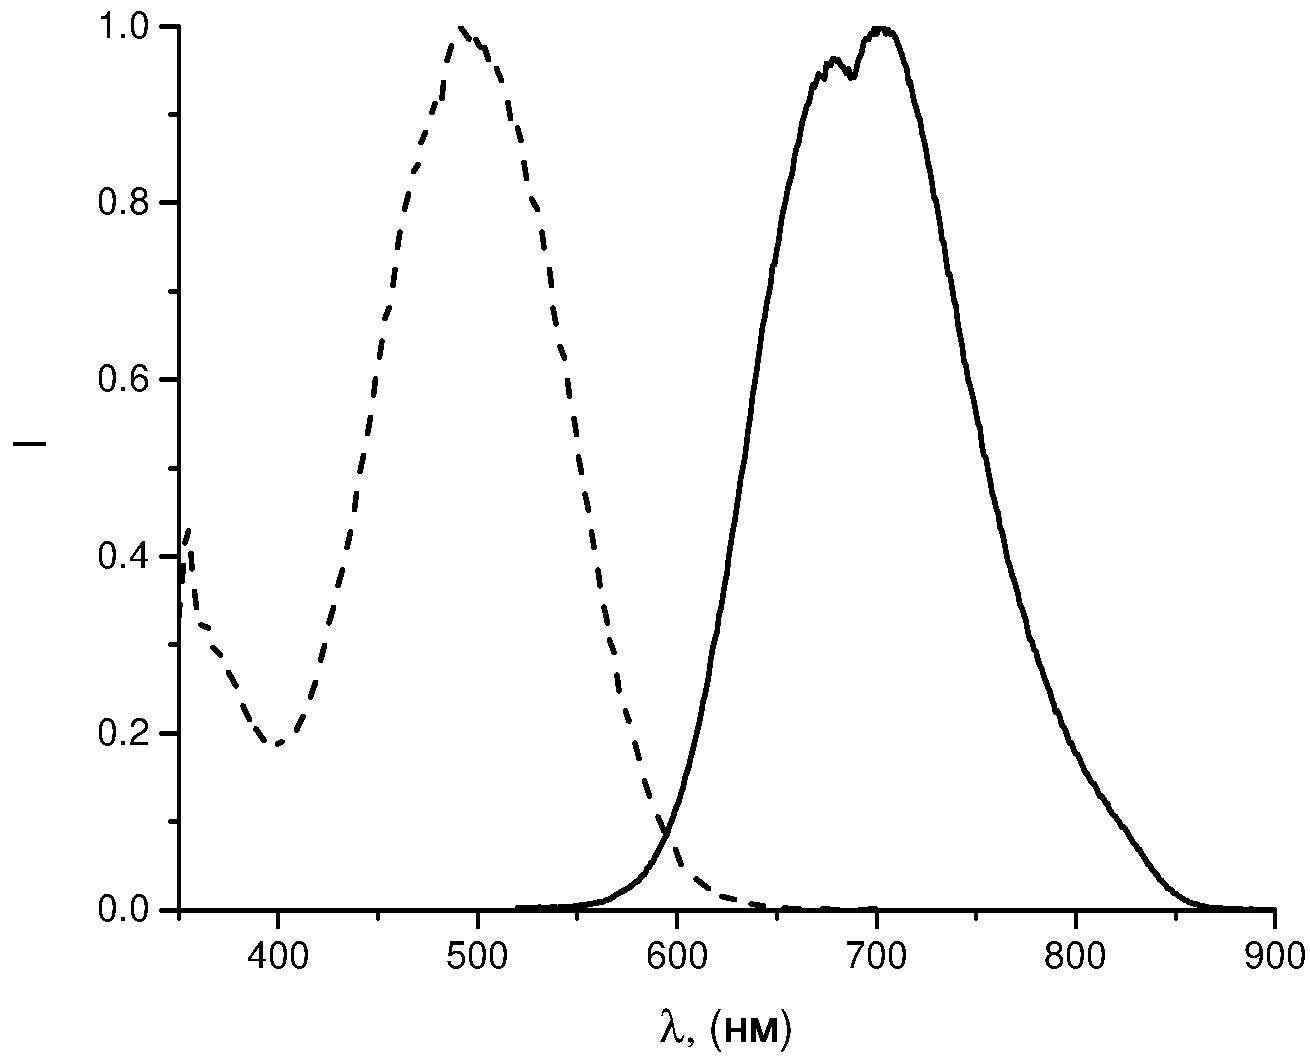
\includegraphics[width = 0.5\textwidth]{sections/results/img/Graph3 - Copy.pdf}
    \caption{Спектры флуоресценции~(сплошная линия) и возбуждения флуоресценции~(пунктирная линия) соединения~\cmpd{decafluoropyrazoline_piperidine_DCIF.TAFS}}
\end{figure} \todo{надо бы еще в разных растворителях}

В спектрах ЯМР~\ce{^1H} соединений~\cmpd{pentafluoropyrazoline_piperidine_DCIF.{TAFS, TATBS, MATBS}} наблюдается сигнал около \SI{4.2}{\ppm}, соответствующий \ce{S-CH2} фрагменту разделительного блока и сигналы около \SI{2.5}{\ppm}, соответствующие ароматическим метильным группам. Для соединений~\cmpd{pentafluoropyrazoline_piperidine_DCIF.{TATBS, MATBS}} при \SI{1.2}{\ppm} в спектре присутствует сигнал \emph{трет}-бутильной группы. Ароматические протоны основного \todo{подобрать слово} кольца в соединениях \cmpd{pentafluoropyrazoline_piperidine_DCIF.{TAFS, TATBS}} проявляются в виде синглета при 7.7--\SI{7.8}{\ppm}. В спектрах соединений~\cmpd{decafluoropyrazoline_piperidine_DCIF.{benzoyl, TAFS, TATBS}} описанные сигналы выглядят как дублеты из-за неэквивалентности двух заместителей. Спектры \ce{^19F} соединений~\cmpd{decafluoropyrazoline_piperidine_DCIF.{TAFS}} и~\cmpd{pentafluoropyrazoline_piperidine_DCIF.{TAFS}} соответствуют структуре TAFS-фрагмента.

% \subsection{Красители с остатком пиперазина}
